\documentclass[aspectratio=169,11pt]{beamer}
\usetheme{Madrid}
\usepackage{amsmath, amssymb}
\usepackage{graphicx}
\usepackage{tikz}
\usepackage{comment}
\usepackage{hyperref}
\usepackage{subcaption}

\title[]{A toy model of deep learning}
\author[Corlouer]{Guillaume Corlouer}
\date{\today}

\begin{document}
\maketitle
\begin{frame}{Motivation 1: Implicit biases of the training process have safety implication}
\begin{itemize}
    \item Parameter $\theta\in \Omega$, input-output data $(Y,X)\sim P$, Neural network $f(\theta, x)$
    \item Degenerate functions: on input $x$ many parameters are compatible with low loss $f(\theta,x)\approx f(\theta',x)$ 
    \item Indinstiguishable on training and eval data
    \item However for some out of distribution input $x_o$, model $f(\theta,x_o)$ is unsafe and $f(\theta',x_o)$ is safe
    \item The data, hyperaparameters, optimization determine if training favour safe or unsafe model
\end{itemize}

\end{frame}

\begin{frame}{Motivation 2: Interpretability over training}
\begin{itemize}
    \item Challenging to know what are principled observables to track
    \item Learning dynamics can help defining useful observables
    \item Challenging to reverse engineer a neural network after training
    \item Structure often emerges sequentially across different timescales
    \item Might be easier to decompose the internal structure of a model during training 
\end{itemize}

\end{frame}
\section{Setup}
\begin{frame}[plain]
\begin{tikzpicture}[remember picture,overlay]
\node[inner sep=0pt] at (current page.center) {%
\begin{beamercolorbox}[wd=.75\paperwidth,sep=1.4em,center,rounded=true,shadow=true]{title}
{\usebeamerfont{title}\Huge Setup}
\end{beamercolorbox}
};
\end{tikzpicture}
\end{frame}
\begin{frame}[plain]
\centering
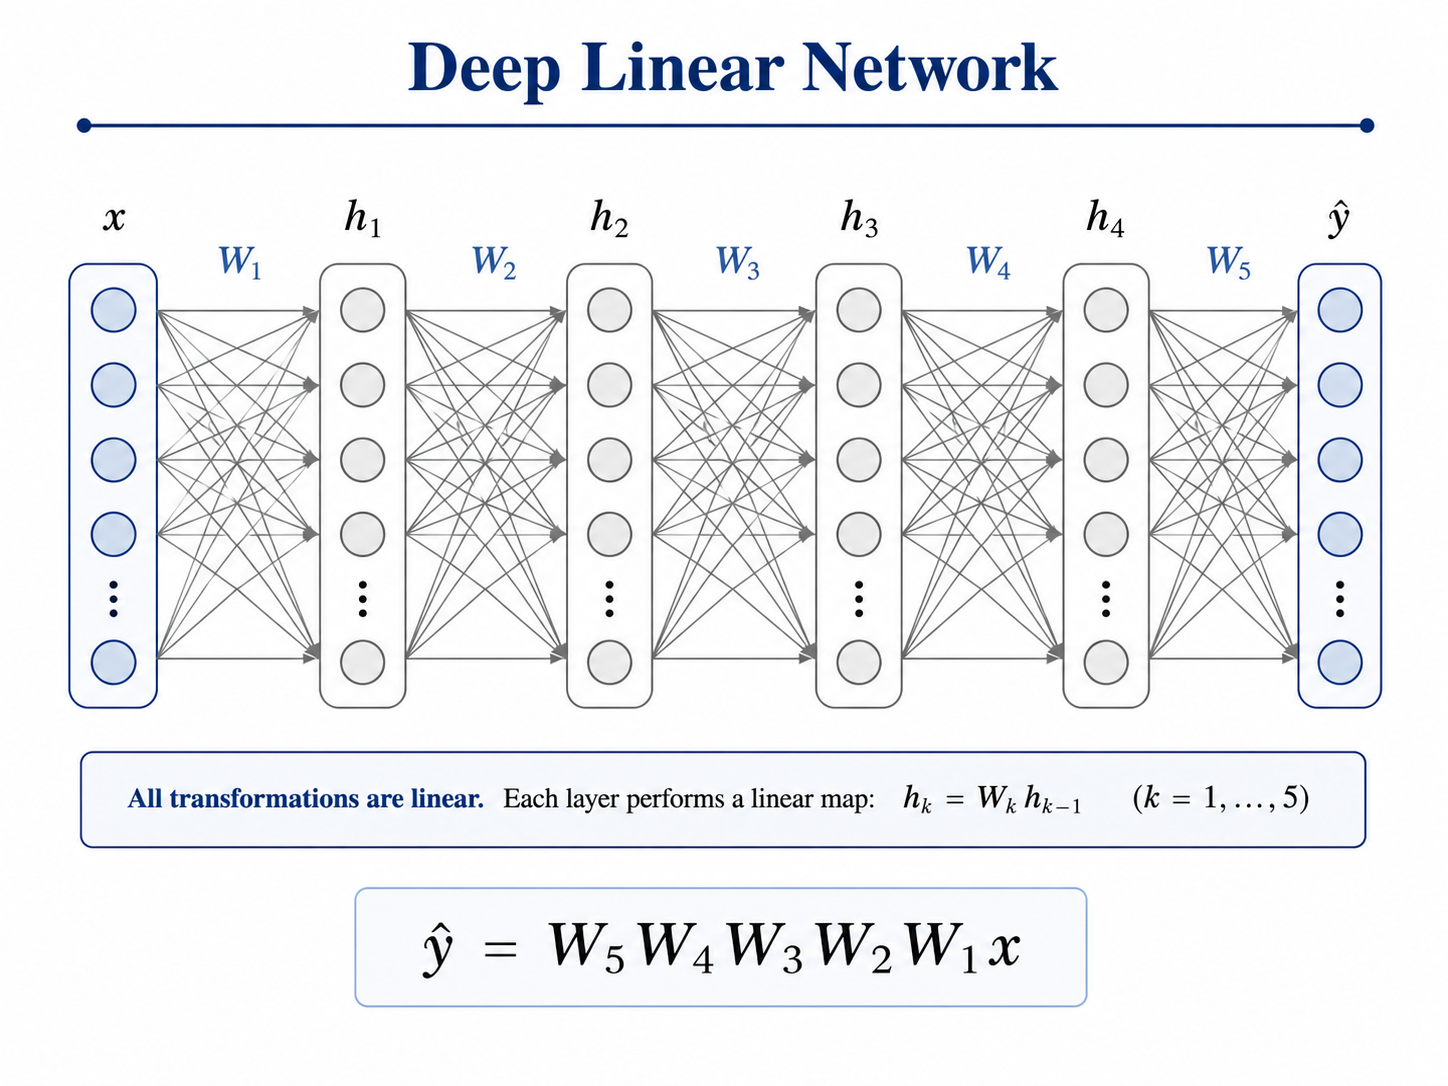
\includegraphics[width=\paperwidth,height=\paperheight,keepaspectratio]{figures/DLN_diagram.png}
\end{frame}
\begin{frame}{The harmonic oscillator of deep learning}
\begin{block}{Definition}
A $L$-layer Deep Linear Network is a function:
\begin{align*}
    f: \ & \mathbb{R}^{d_0}\times \prod_{l=1}^{L-1}\operatorname{Mat}_{d_l\times d_{l-1}}  \to \mathbb{R}^{d_L} \\
       & (x,\theta :=(W_1,...,W_L)) \mapsto W_L...W_1 x = Wx
\end{align*}
$d_0$: dimension of the input data; $d_l,\ 1\leq l \leq L$: width of layer $l$ student matrix $W$. 
\end{block}
DLN: multi-linear function, linear in $W_l$ and in the input data $x$ and linear in $W$.
\end{frame}
\begin{frame}[plain]
\centering
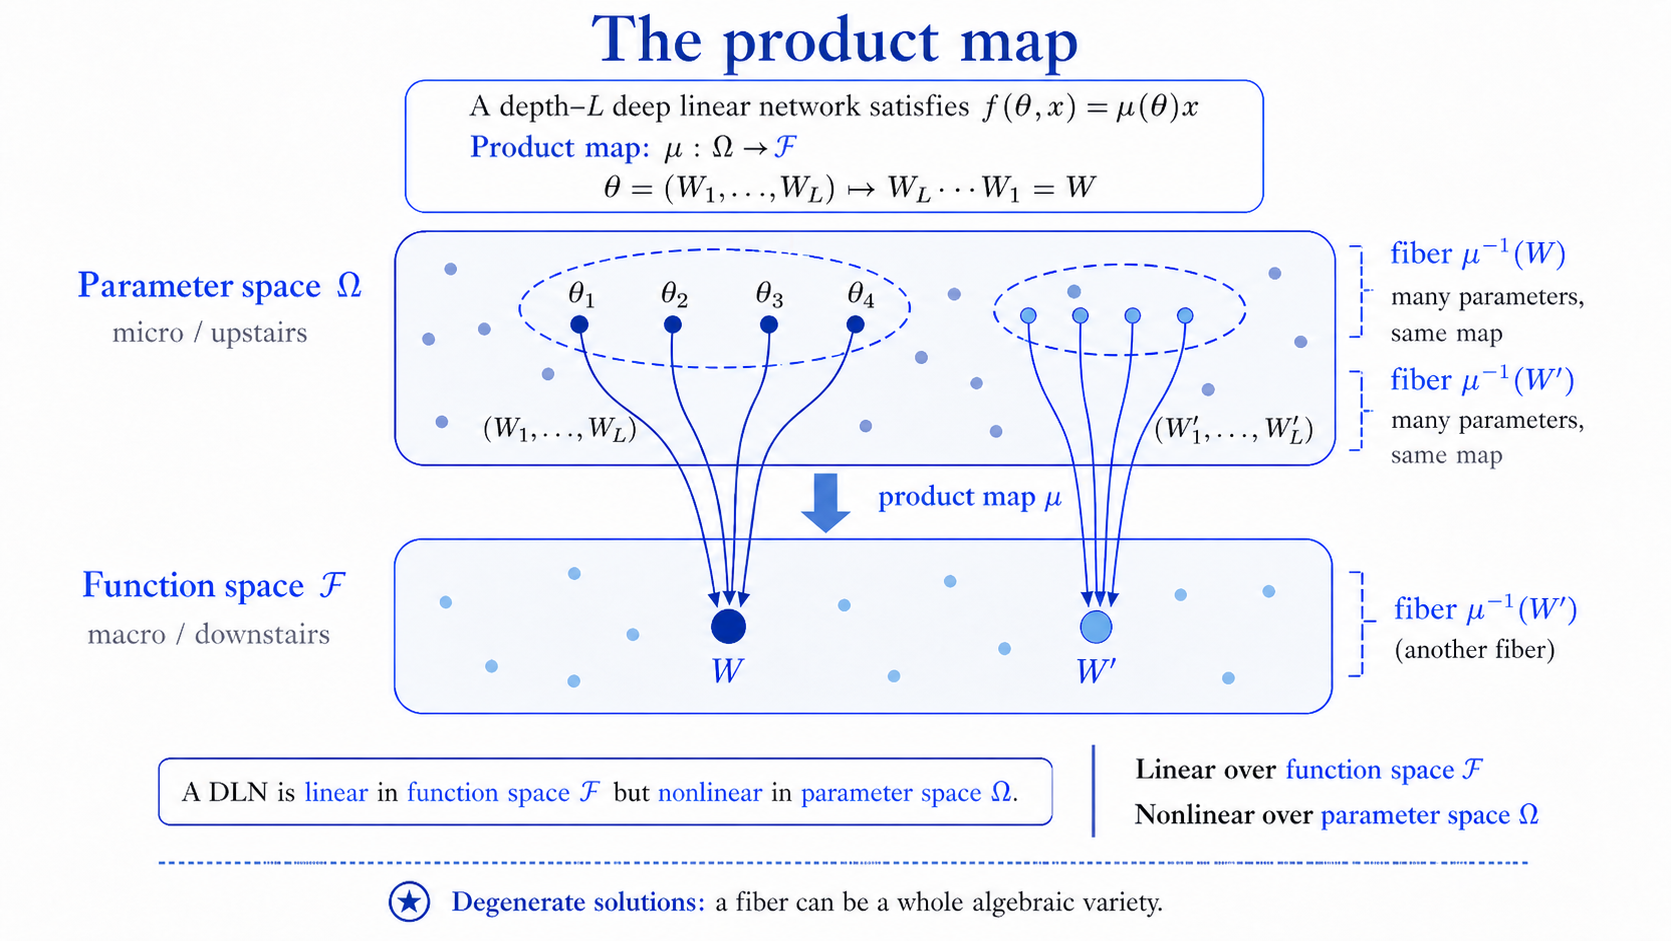
\includegraphics[width=\textwidth,height=\textheight,keepaspectratio]{figures/DLN_fiber_mult_map.png}
\end{frame}
\begin{comment}
% ---------- Slide: Product map----------
\begin{frame}{The product map}
\begin{block}{Definition}
A DLN $f(\theta,x)$ of depth $L$ satisfies $f(\theta,x)= \mu(\theta)x$ with \textit{product map} $\mu$:
    \begin{align*}
    \pi :  & \ \Omega = \operatorname{Mat}_{d_l\times d_{l-1}}\to \mathcal{F} = \operatorname{Mat}_{d_0\times d_L}\\
         \theta:=& (W_1,...,W_L) \mapsto W_L...W_1=W
\end{align*}
We note $W:=\pi(\theta)$. A DLN is linear over function space $\mathcal{F}$ and non-linear over parameter space $\Omega$.
\end{block}
Intuition: Parameter space $\Omega$ is micro (upstair) and $\mathcal{F}$ is macro (downstair). 
\\
Degenerate solutions: fiber $\mu^{-1}(\theta)$ can be a whole algebraic variety.
\end{frame}
\end{comment}
\begin{frame}{Data,  loss function, training}
\begin{block}{Quadratic Population loss and gradient flow}
Teacher matrix $M$ such that $y=Mx$ for $x$ generated by $N(0,I)$ distribution. 
Input-output covariance $\Sigma_{YX}=M$ 
\begin{equation*}
    \mathcal{L}(\theta) : = \frac{1}{2} ||(M - W_L...W_1)||^2_F = \frac{1}{2} ||(M - W)||^2_F
\end{equation*}
Initialize $\theta_0 \sim N(0, \sigma^{-\gamma})$ with $\gamma$ init. scale, then gradient flow:
\[
\dot{W}_l = - \nabla_{W_{l}} L(\theta)
\]
\end{block}
Frobenius norm as $||A||_F:=\sqrt{\text{Tr}(A^{\top}A)}$
\\
Global minimizer achieving zero loss: $\exists \theta^{\star}\in \Omega,\ \mu(\theta^{\star}) = \ W^{\star} = M$ 
\\
Structure of the data encoded by $\Sigma_{YX}$

\end{frame}
\begin{frame}
    \centering Empirical phenomena
\end{frame}

\begin{frame}{Training losses}
    \begin{figure}
        \centering
        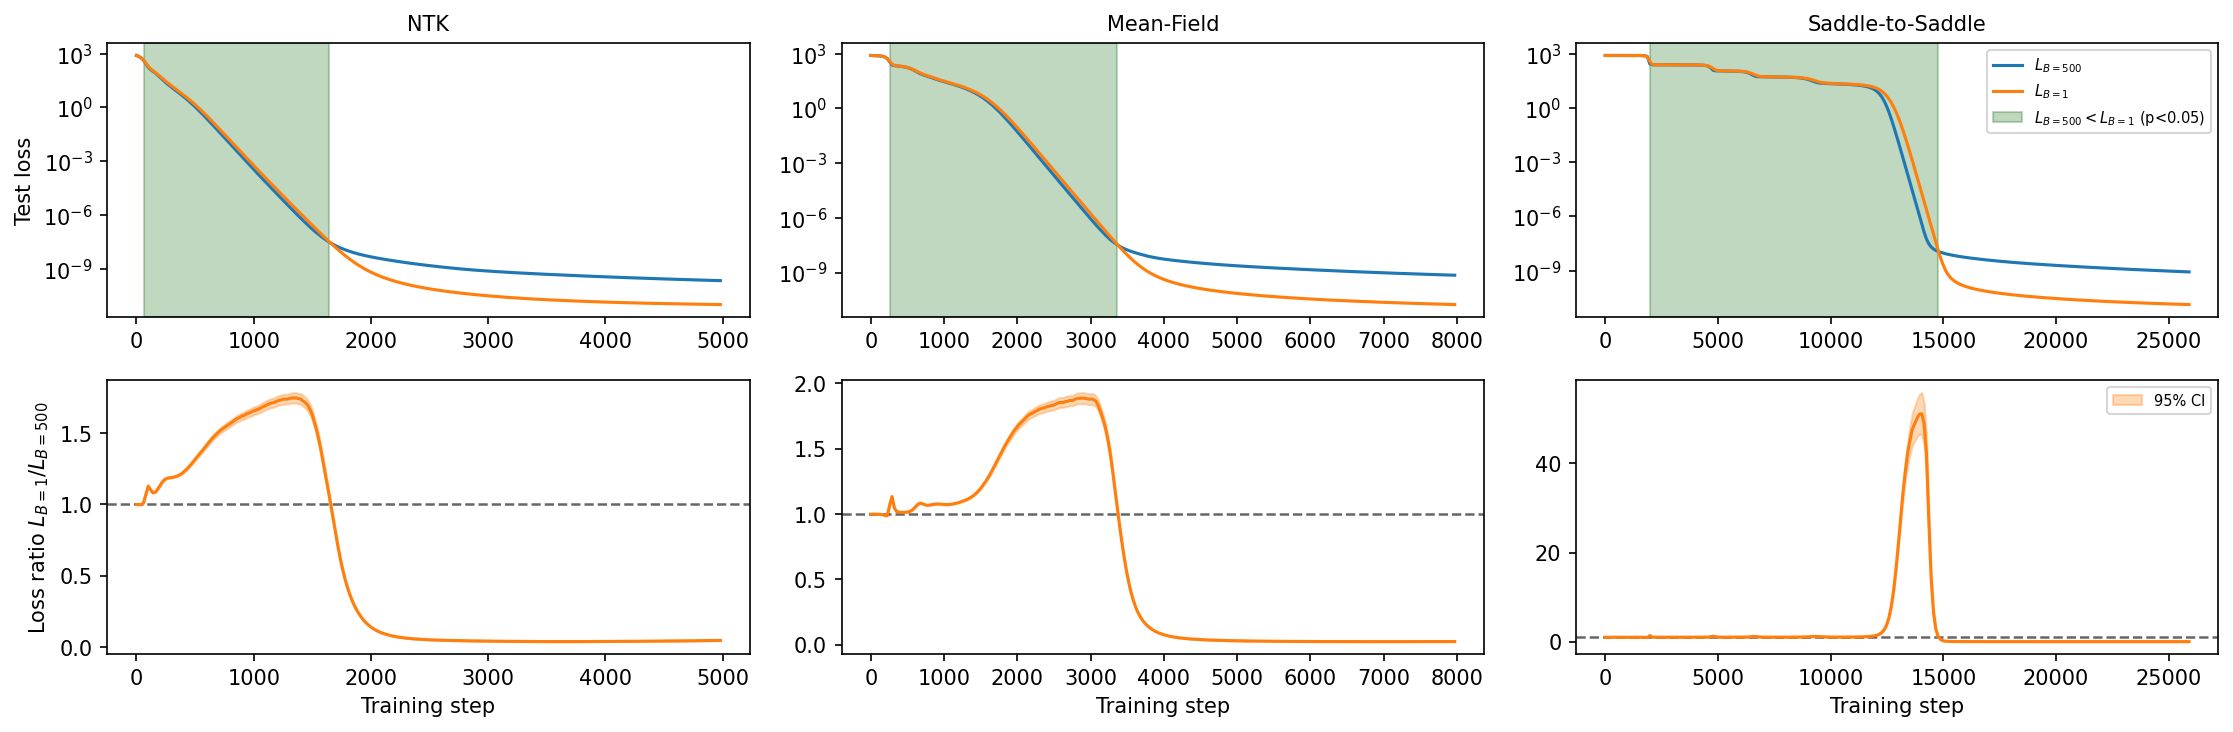
\includegraphics[width=\linewidth]{figures/DLN_losses_regimes.png}
    \end{figure}
\end{frame}

\begin{frame}{Singular values of student matrix}
    \begin{figure}
        \centering
        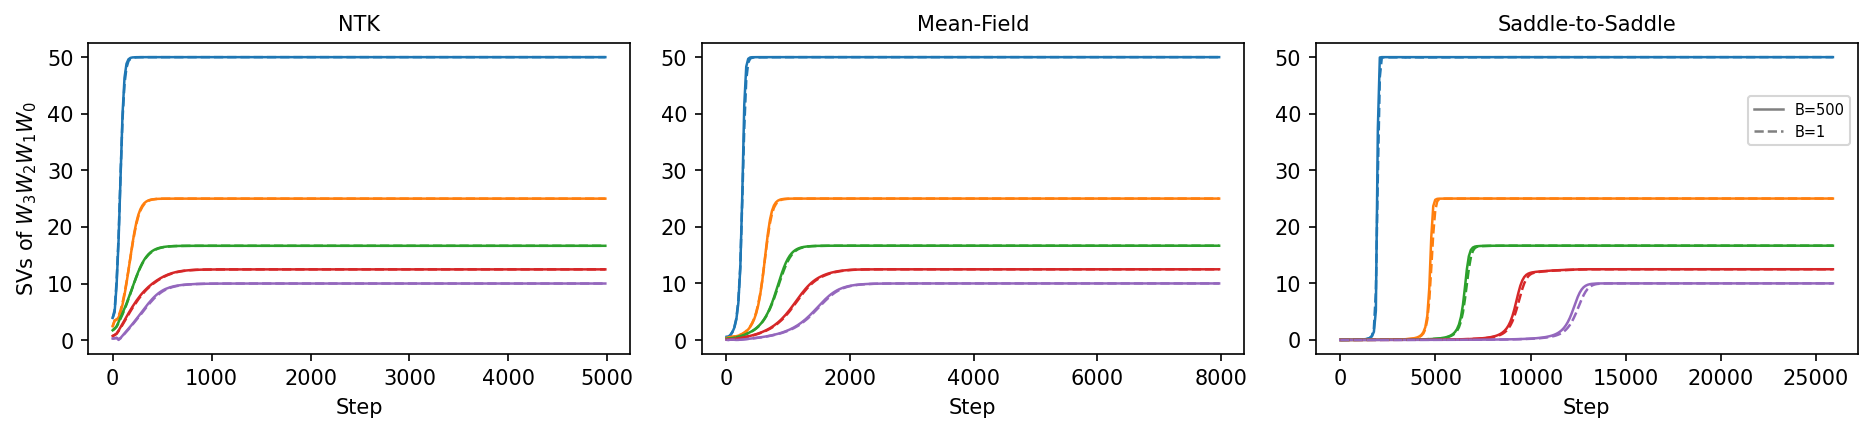
\includegraphics[width=\linewidth]{figures/DLN_sv_students.png}
    \end{figure}
\end{frame}

\begin{frame}{Singular values of individual weight matrices}
    \begin{figure}
        \centering
        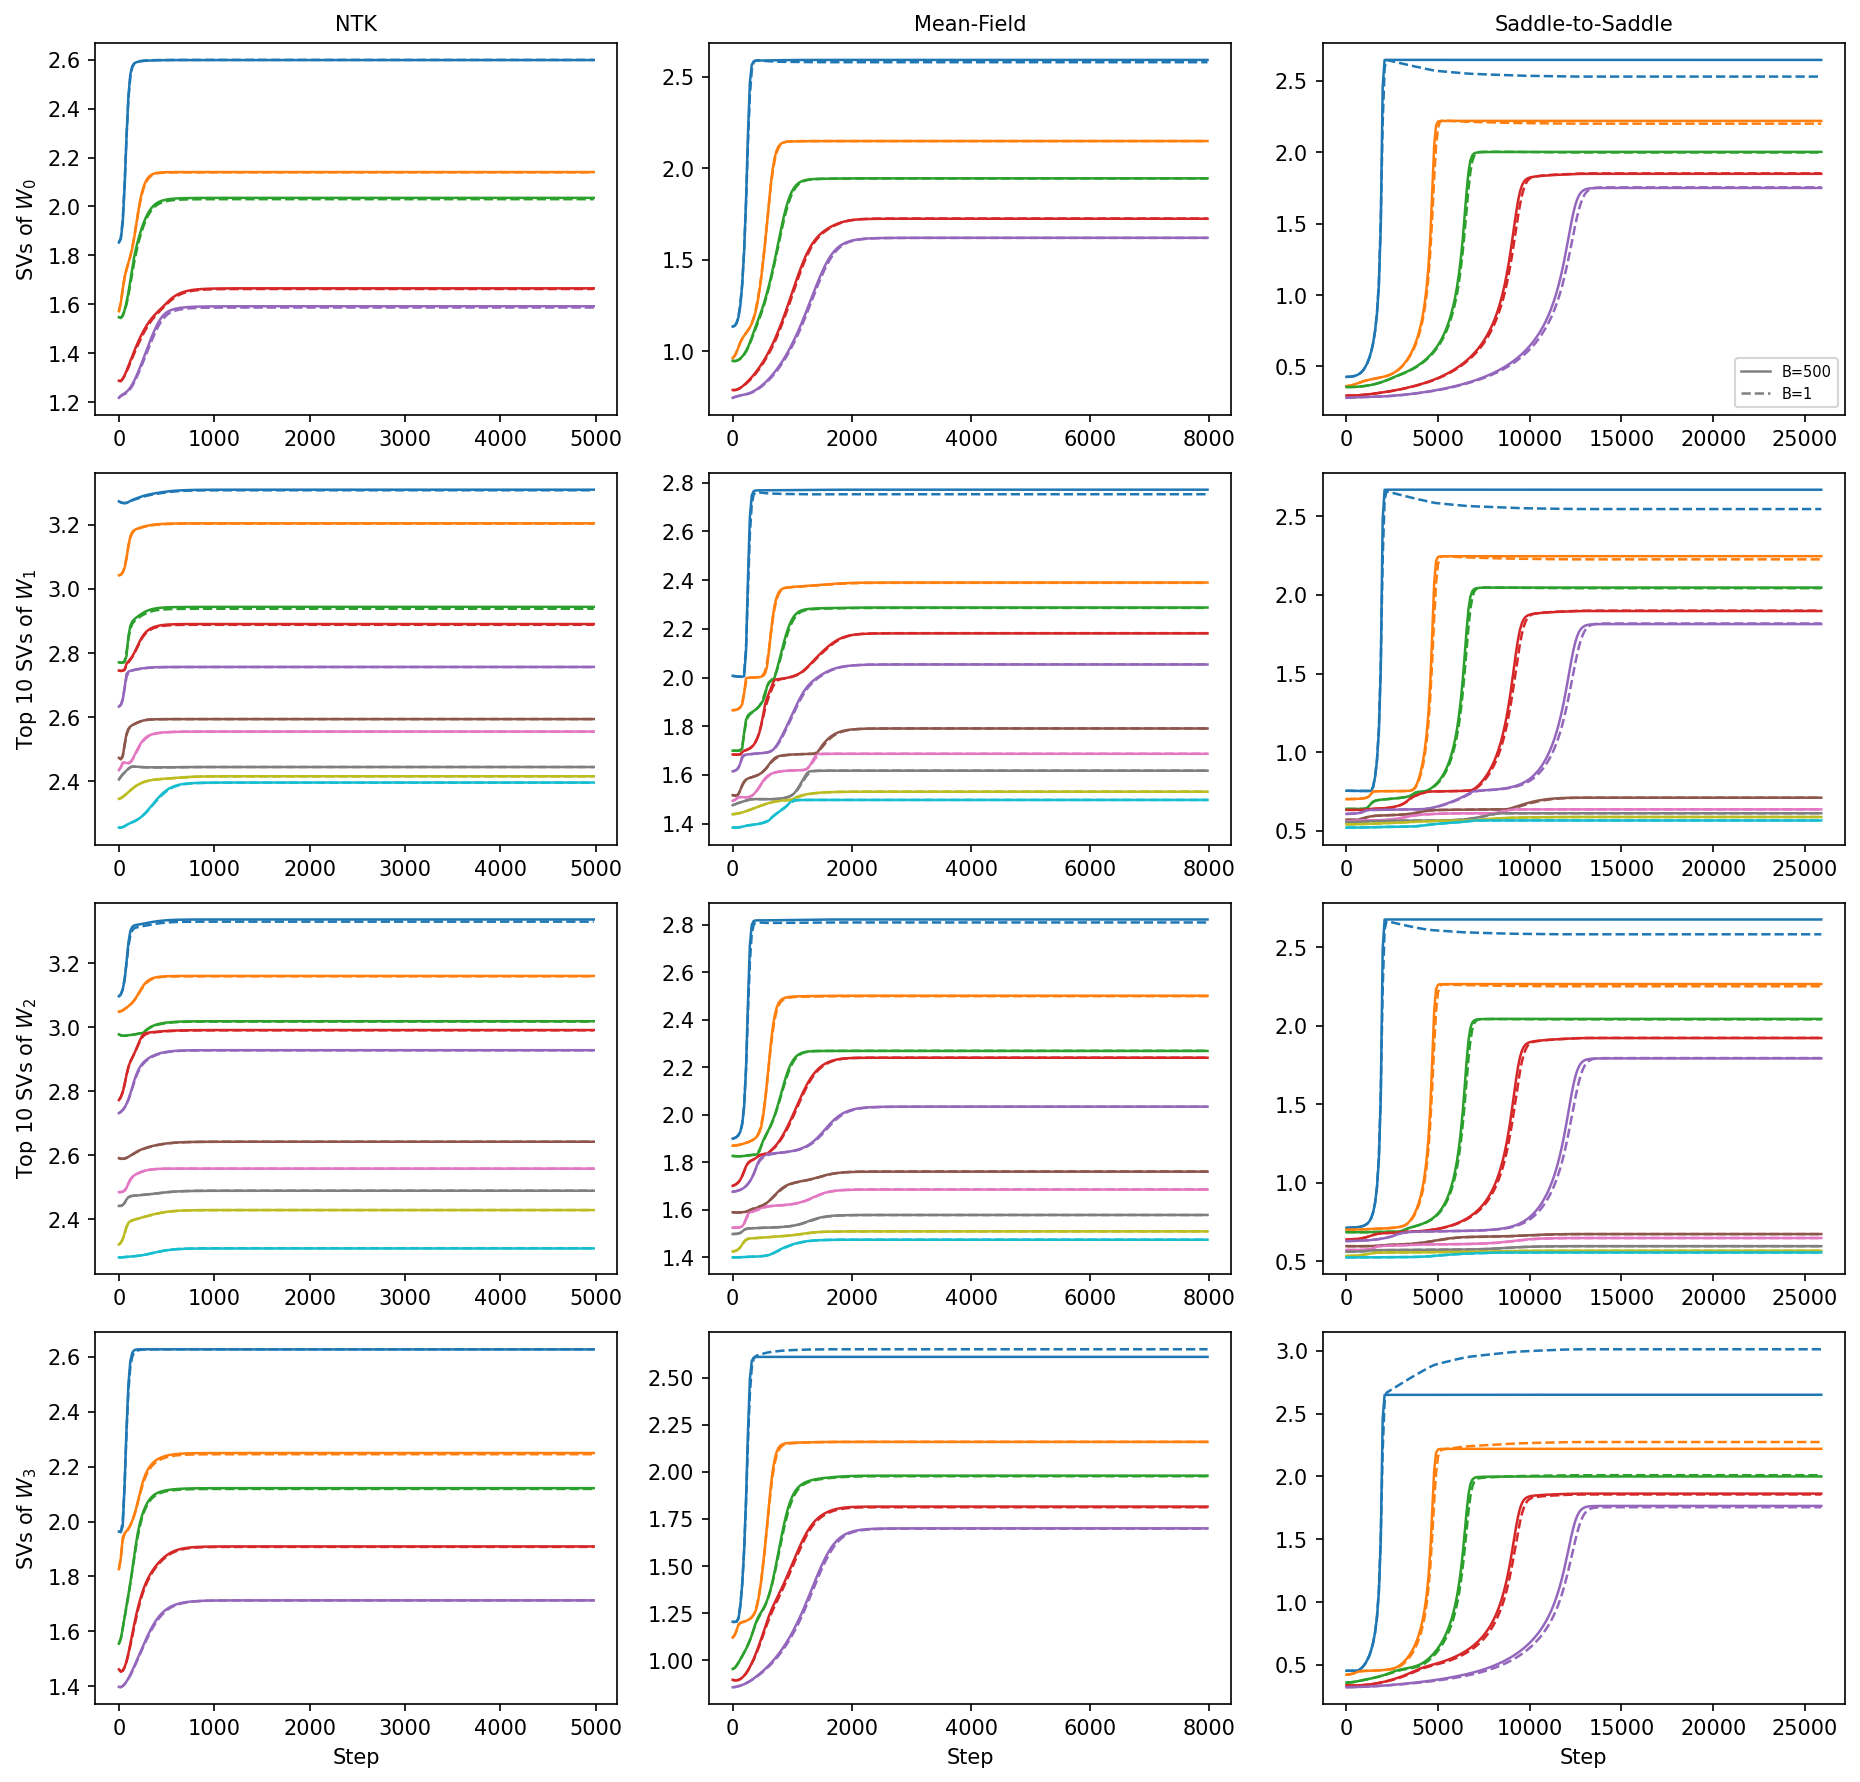
\includegraphics[width=\linewidth]{figures/DLN_individual_sv.png}
    \end{figure}
\end{frame}
\begin{frame}
    \centering Geometry
\end{frame}
% ---------- Slide: 2-layer diagonal DLN ----------
\begin{frame}{A 2-layer diagonal DLN}

\begin{block}{Model and loss}
Take a 2-layer diagonal DLN of width \(2\):
\[
W_1=\operatorname{diag}(b_1,b_2),
\qquad
W_2=\operatorname{diag}(a_1,a_2),
\qquad
\theta=(W_1,W_2).
\]
Hence the student matrix is
\[
W=W_2W_1=\operatorname{diag}(a_1b_1,a_2b_2).
\]
Let the teacher be
\[
M=\operatorname{diag}(s_1,s_2),
\qquad s_1,s_2>0,
\qquad x\sim \mathcal N(0,I).
\]
With whitened inputs, the quadratic population loss is
\[
\mathcal L(\theta)
=
\frac12\|M-W\|_F^2
=
\frac12(a_1b_1-s_1)^2
+
\frac12(a_2b_2-s_2)^2.
\]
\end{block}
\end{frame}
\begin{frame}
\begin{block}{Gradient equations}
For \(i=1,2\),
\[
\partial_{a_i}\mathcal L
=
(a_i b_i-s_i)b_i,
\qquad
\partial_{b_i}\mathcal L
=
(a_i b_i-s_i)a_i.
\]
Therefore the critical point equations are
\[
(a_i b_i-s_i)b_i=0,
\qquad
(a_i b_i-s_i)a_i=0,
\qquad i=1,2.
\]
\end{block}

\centering
\small
The two coordinates decouple: each singular direction can be analyzed independently.

\begin{block}{Coordinate-wise characterization}
For each \(i=1,2\), the critical point equations are
\[
(a_i b_i-s_i)b_i=0,
\qquad
(a_i b_i-s_i)a_i=0.
\]
Since \(s_i>0\), this implies exactly two possibilities:
\[
a_i b_i=s_i
\qquad\text{or}\qquad
a_i=b_i=0.
\]
Thus each coordinate either fits the teacher singular value or is shut off.
\end{block}

\end{frame}


% ---------- Slide: Critical points ----------
\begin{frame}{Critical points}

\begin{block}{All critical points}
\[
\begin{array}{c|c|c}
\text{Parameter conditions}
&
\text{Realized student matrix } W
&
\text{Loss}
\\
\hline
a_1b_1=s_1,\ a_2b_2=s_2
&
W=\operatorname{diag}(s_1,s_2)=M
&
\mathcal L=0
\\[0.4em]
a_1b_1=s_1,\ a_2=b_2=0
&
W=\operatorname{diag}(s_1,0)
&
\mathcal L=\frac12s_2^2
\\[0.4em]
a_1=b_1=0,\ a_2b_2=s_2
&
W=\operatorname{diag}(0,s_2)
&
\mathcal L=\frac12s_1^2
\\[0.4em]
a_1=b_1=0,\ a_2=b_2=0
&
W=0
&
\mathcal L=\frac12(s_1^2+s_2^2)
\end{array}
\]
\end{block}

\centering
\small
Critical points correspond to choosing a subset of the teacher singular values. 
\\
Depth introduces three new critical points compared with the one layer DLN loss $L(W)=||M - \text{diag}(w_1,w_2)||^2_F$ 

\end{frame}


% ---------- Slide: Saddles or global minimum ----------
\begin{frame}{Global minimum and saddles}

\begin{block}{Example}
If both singular directions are fitted,
\[
a_1b_1=s_1,
\qquad
a_2b_2=s_2,
\]
then
\[
W=M=\operatorname{diag}(s_1,s_2),
\qquad
\mathcal L=0.
\]
Since \(\mathcal L(\theta)\geq 0\), these critical points are global minima.
\end{block}
\end{frame}
\begin{frame}[plain]
\centering
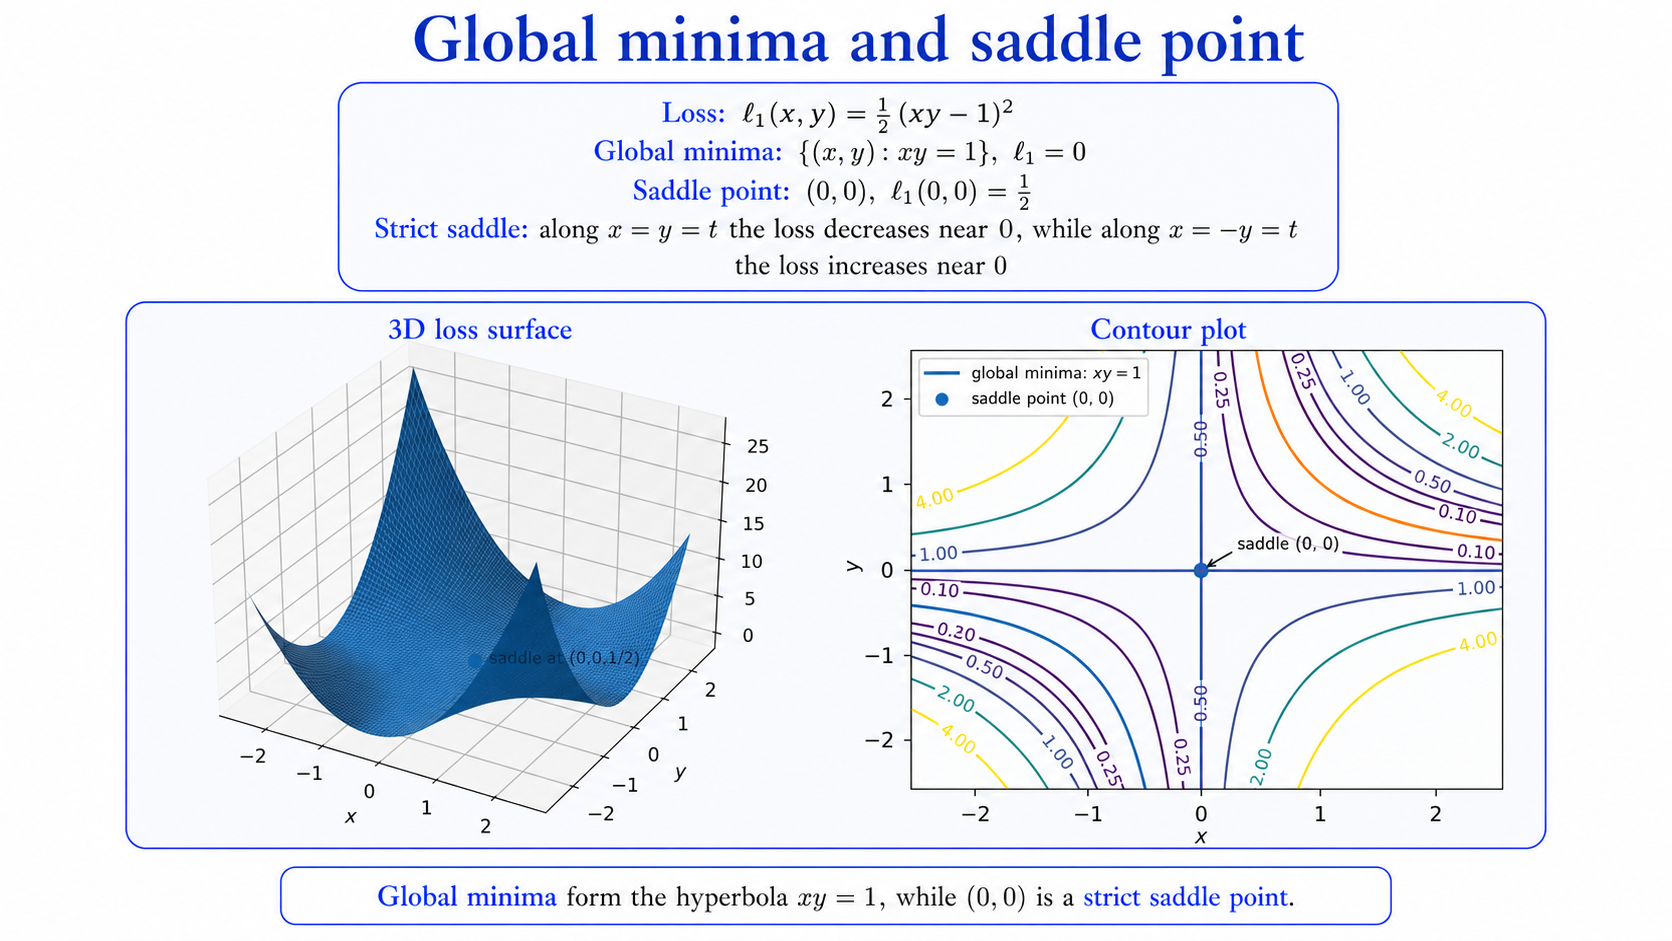
\includegraphics[width=\textwidth,height=\textheight,keepaspectratio]{figures/global_minima_saddle_3d_loss.png}
\end{frame}
\begin{comment}
\begin{frame}
\begin{block}{Example: \(W=\operatorname{diag}(s_1,0)\) is a saddle}
Take a critical point with \(a_1b_1=s_1\) and \(a_2=b_2=0\).

For the perturbation \(a_2=t,\ b_2=t\),
\[
W(t)=\operatorname{diag}(s_1,t^2),
\]
and
\[
\mathcal L(t)-\mathcal L(0)
=
\frac12(t^2-s_2)^2-\frac12s_2^2
=
-s_2t^2+\frac12t^4<0
\]
for small \(t\neq 0\).

For the perturbation \(a_2=t,\ b_2=-t\),
\[
W(t)=\operatorname{diag}(s_1,-t^2),
\]
and
\[
\mathcal L(t)-\mathcal L(0)
=
\frac12(-t^2-s_2)^2-\frac12s_2^2
=
s_2t^2+\frac12t^4>0.
\]
Thus there are both descending and ascending directions, so this critical point is a saddle.
\end{block}
\end{frame}
\end{comment}
\begin{frame}{Deep learning without poor local minima}
Assume that $\Sigma_X$ and $\Sigma_{YX}$ are full rank. Assume that $\Sigma_{YX}$ has $d_L$ distinct singular values. 
\begin{block}{No non-global local minima}
    The loss function of DLN of depth $L$ is non-convex, non-concave, and every critical point that is not a global minimum is a saddle point. 
\end{block}
The training dynamics cannot get stuck in spurious local minima. 
\\
Reference: \textit{Kawaguchi, Kenji. "Deep learning without poor local minima." Advances in neural information processing systems 29 (2016)}
\end{frame}
\begin{frame}{Parametrization of critical points}
Teacher SVD: \(M=U\operatorname{diag}(s_1,...,s_{r_m},0_{d_L-r_m})V^{\top}\).
\begin{block}{Saddle points}
    Let $\theta\in\Omega$ be a critical point of rank $r$. Then there exists a subset $S$ of left singular vector of $M$ and a projector $P_S=U_SUS^{\top}$ over these singular vector such that:
    \[
    \mu(\theta) = P_SM = U_S\operatorname{diag}(s_1,...,s_{r},0_{d_L-r})V^{\top}
    \]
\end{block}
The saddle points are given by a subset of singular values and (left) singular vectors of the teacher $M$.
\\
Reference: \textit{Achour, El Mehdi, François Malgouyres, and Sébastien Gerchinovitz. "The loss landscape of deep linear neural networks: a second-order analysis." Journal of Machine Learning Research 25.242 (2024): 1-76.}
\end{frame}
\begin{frame}{Symmetries}
Let $G_{\textbf{d}}:=\Pi_{l=L}^0 GL_{d_l} = GL_{d_L}\times GL_{h} \times GL_{d_0}$ acts on $\Omega$ via:
\[
(W_1,\dots,W_L)\mapsto (g_1W_1g_0^{-1},\; g_2W_2g_1^{-1},\;\dots,\; g_L W_L g_{L-1}^{-1}),
\]
\begin{block}{Equivariance of the multiplication map}
    Since \(W_Lg_{L-1}^{-1}g_{L-1}W_{L-2}g_{L-2}^{-1}...g_1W_1=W_L...W_1\), the multiplication map $\mu$ is $GL_{\textbf{d}}$-equivariant and $G_h$-invariant i.e.: $$\mu(g\cdot \theta)=g_LWg_0^{-1};\quad \mu(g_h\cdot \theta) = \mu(\theta) $$
A DLN is degenerate and there are infinite DLNs that maps to a particular student.
\end{block}
Natural to study solutions up to $G_d$ symmetries: by equivariance of $\mu$ we have a group action of $G_d$ over the determinental variety $G_{\text{out}}.\mu^{-1}(\theta)=\Sigma_d^{r}:=\{\theta\in \Omega|\operatorname{rank}(\mu(\theta)) = r\}$    
\end{frame}
\begin{comment}
\begin{frame}{Quiver representation theory}
    \begin{block}{Basic notions}
    A quiver $Q$ is a graph $(I,E,s,t)$ with a map $s(e) = V_{i}$ and $t(e)=V_{i+1}$ when edge $e\in E$ connects vertices $i$ and $i+1$ in $I$. Loops and cycles are allowed.
    \\
    A quiver representation assigns a vector space $V_i$ to each $i\in I$ and a linear map $\phi_e$ to each arrow $e\in E$. Note $\text{Rep}_d(Q)$ the space of representations of dimension vector $d=(d_i)_{i\in I}$ 
    \end{block}
Example: The linear quiver $A_n:1\to 2\to ... \to n$ and representation $k\to^{id} k \to^{id} ... \to^{id} k$
\begin{block}{DLN as quiver representations}
The multiplication map of a DLN $\mu$ is a map from $\text{Rep}_d(A_{L+1})\to \operatorname{Mat}_{d_L\times d_0}$ with linear maps given by weight matrices $W_i$ and vector space $\mathbb{R}^{d_i}$. 
\end{block}
In particular $\Sigma_d^r$ is a subvariety of $\text{Rep}_d(A_{L+1})$.
\end{frame}
\end{comment}
\begin{frame}[plain]
\centering
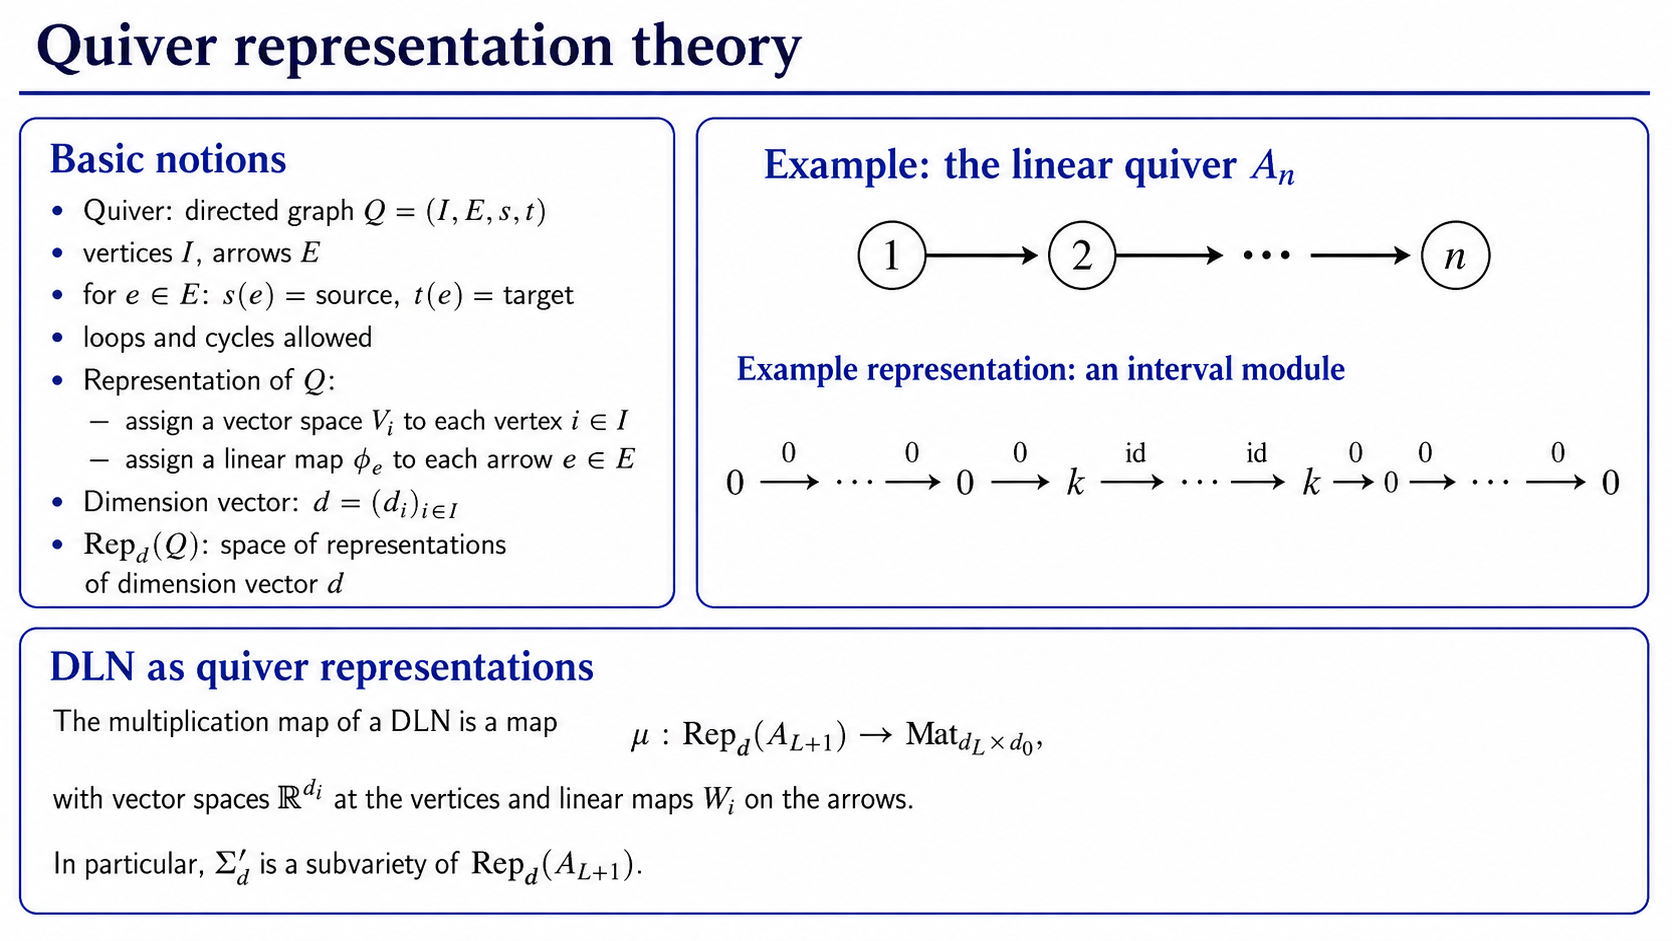
\includegraphics[width=\textwidth,height=\textheight,keepaspectratio]{figures/quiver_representation_theory.png}
\end{frame}
\begin{frame}[plain]
\centering
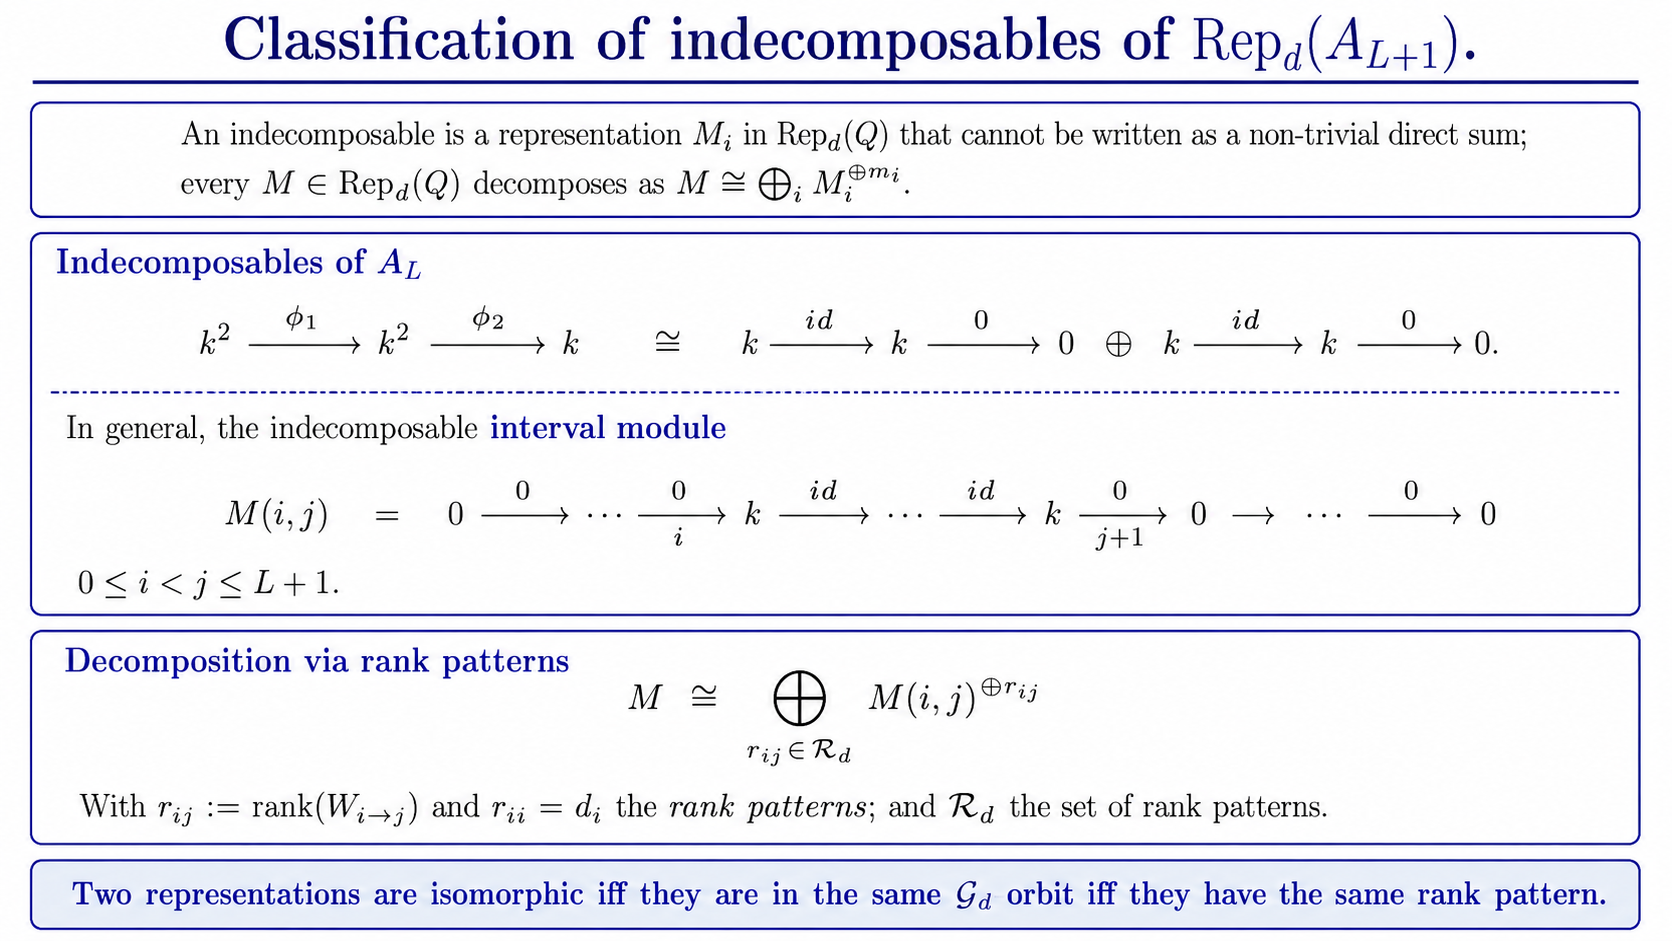
\includegraphics[width=\textwidth,height=\textheight,keepaspectratio]{figures/indecomposables_linear_quiver.png}
\end{frame}
\begin{comment}
\begin{frame}{Classification of indecomposables of ${Rep}_d(A_{L+1})$}
Indecomposable is smallest $M_i \in \text{Rep}_d(Q) $ such that $M \cong \bigoplus M_i^{m_i}$ for $M\in\text{Rep}_d(Q)$ 
\begin{block}{Indecomposables of $A_L$}
Example: $k^2 \to^{\phi_1} k^2 \to^{\phi_2} k \cong k \to^{id} k \to^0 0 \oplus k \to^{id} k \to^0 0$.
\\
More generally all indecomposables are of the form:
$M(i,j) = 0\to^{0} ... \to^{0}_i k \to^{id} ... \to^{id} k \to^{0}_{j+1} 0 \to ... \to^{0} 0 $ for $0\leq i < j \leq L + 1$ 
\\
See: Gabriel Theorem for Dynkin quivers.     
\end{block}
\begin{block}{Decomposition via rank patterns}
Krull-Schmidt and Gabriel theorem $\implies$ for all $M\in \text{Rep}_d(A_{L+1})$ we have a unique decomposition:
\[
M \cong \bigoplus_{r_{ij}\in \mathcal{R}_d} M(i,j)^{\oplus r_{ij}}
\]
With $r_{ij} := \operatorname{rank}(W_{i\to j})$ and $r_{ii}=d_i$ the \textit{rank patterns}; and $\mathcal{R}_d$ the set of rank patterns (with some constraints)
\end{block}
\end{frame}
\end{comment}
\begin{frame}{Stratification of the detreminental variety}
\begin{block}{Orbits are parameterized by rank patterns}
We have $G_d$ action over $\Sigma_d^r$ hence:
\[
\Sigma_d^r = \bigsqcup_{\rho\in R^r_d} \mathcal O_{\rho}
\] 
Two representations are in the same $G_d$-orbits iff they are isomorphic iff they have the same decomposition into indecomposable. So:
\[
\Sigma_d^r = \bigsqcup_{\rho\in \mathcal{R}^r_d} \mathcal O_{\rho}
\]
We have a stratification in the geometric sense: $G_d$-orbits parameterized by rank patterns stratify $\Sigma_d^r$
\\
Since $\Sigma_d^{r_m} =G_{\text{out}}\cdot\mu^{-1}(M)$ this gives a combinatorial description of the global minima.
\end{block}
The rank patterns are natural geometric invariants observables for DLNs.   
\end{frame}
\begin{frame}{Link with SLT}
\begin{block}{Codimension of global minima}
For teacher matrix $M$ of rank $r_m$ we have:
    \[
    \text{codim}_{\text{Rep}_d}(\mu^{-1}(M)) = \text{codim}_{\text{Rep}_d}(\Sigma_d^{r_m}) + r_m(d_0 - d_L -r_m) = 2\operatorname{RLCT}(\mathcal{L}^{-1})(0)
    \]
In general we only have:
\[
\operatorname{RLCT}(\mathcal{L}^{-1})(0)  \leq \frac{1}{2}\text{codim}_{\text{Rep}_d}(\mathcal{L}^{-1}(0))
\]
\end{block}
DLN are ``midly'' singular.\\
Ref: \textit{Lehalleur, Simon Pepin, and Richárd Rimányi. "Geometry of fibers of the multiplication map of deep linear neural networks." arXiv preprint arXiv:2411.19920 (2024).}
\end{frame}
\begin{frame}{Discussion}
\begin{block}{Takeaways}
Under assumptions of full rank and non degenerate data:
    \begin{itemize}
        \item Critical points of DLNs are either saddles or global minima
        \item Gauge symmetries means a whole algebraic variety of degenerate minima
        \item Using quiver representation theory we get a combinatorial description of the global minima 
        \item The Codimension of the global minima is twice the RLCT
    \end{itemize}
\end{block}
\begin{block}{Open problems}
    \begin{itemize}
        \item Loss landscapes of non linear networks (ReLU)
        \item Geometric invariants for non linear networks
        \item Combinatorial description of all critical points (work in progress)
    \end{itemize}
\end{block}
\end{frame}
\begin{frame}
    \begin{center}
        Dynamics 
    \end{center}
\end{frame}
\begin{frame}{Gradient Flow}
\begin{block}{Two-layer DLN}
\begin{align*}
    W &:= W_2W_1, &
    R(W) &:= \Sigma_{YX}-W_2W_1 .
\end{align*}

For the population loss
\[
    \mathcal{L}(W_1,W_2)=\frac{1}{2}\|\Sigma_{YX}-W_2W_1\|_F^2,
\]
gradient flow is
\begin{align*}
    \dot{W}_1 &= W_2^{\top}R(W),\\
    \dot{W}_2 &= R(W)W_1^{\top}.
\end{align*}
\end{block}
\end{frame}
\begin{frame}[plain]
\centering
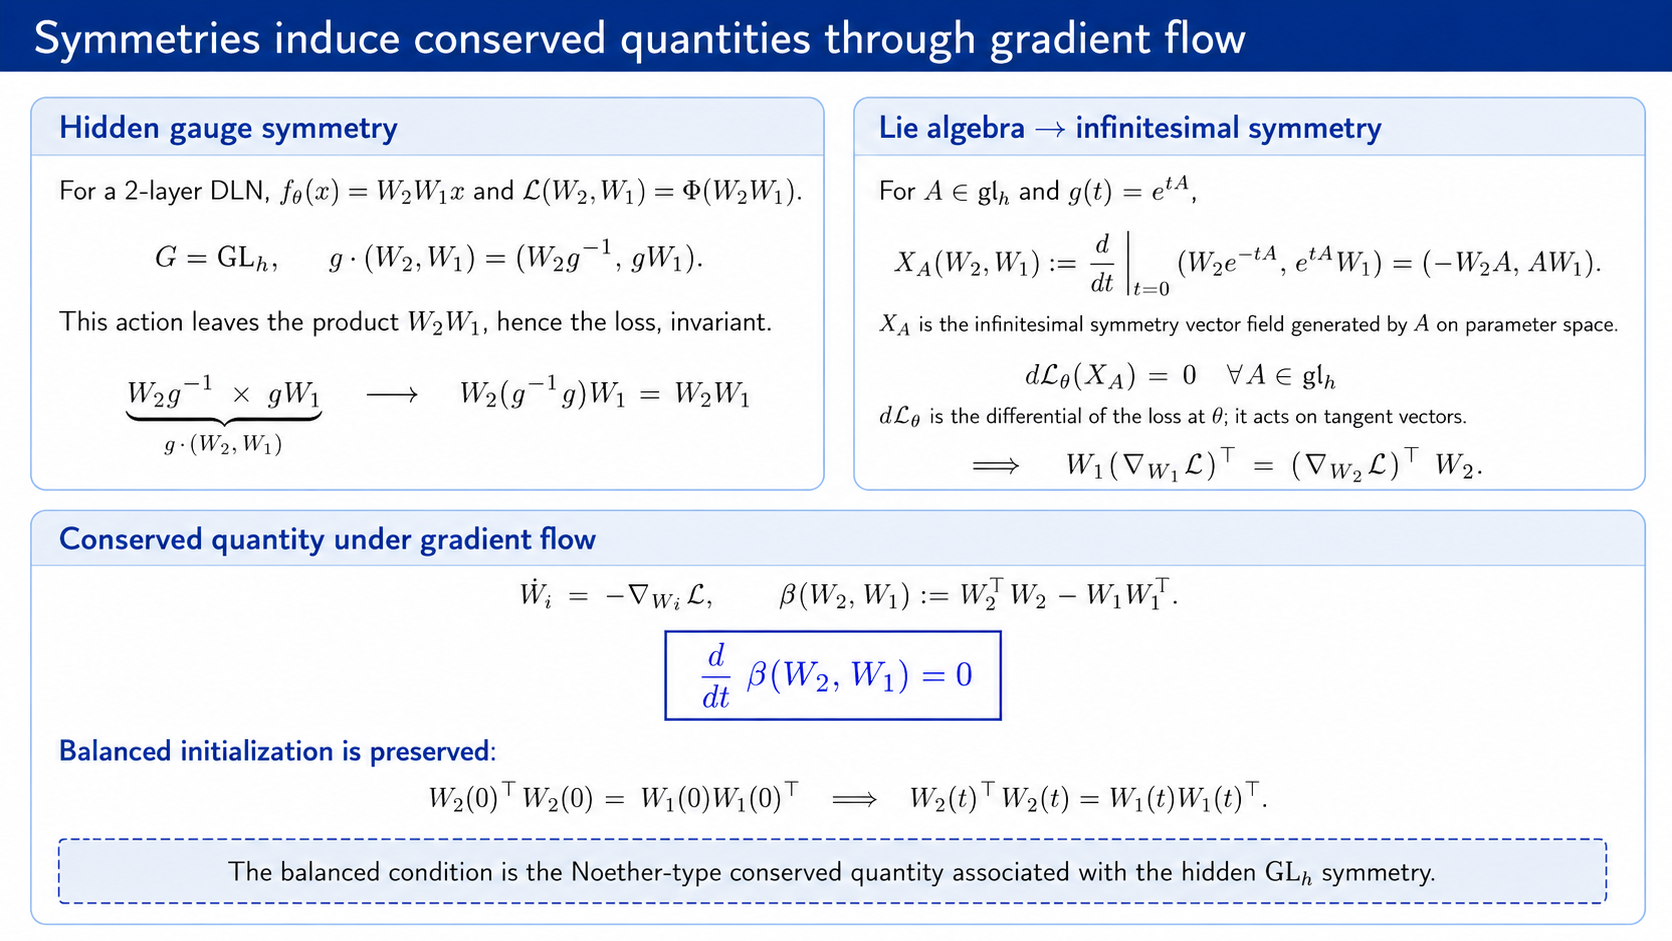
\includegraphics[width=\paperwidth,height=\paperheight,keepaspectratio]{figures/conserved_quantities.png}
\end{frame}
\begin{frame}[plain]
\centering
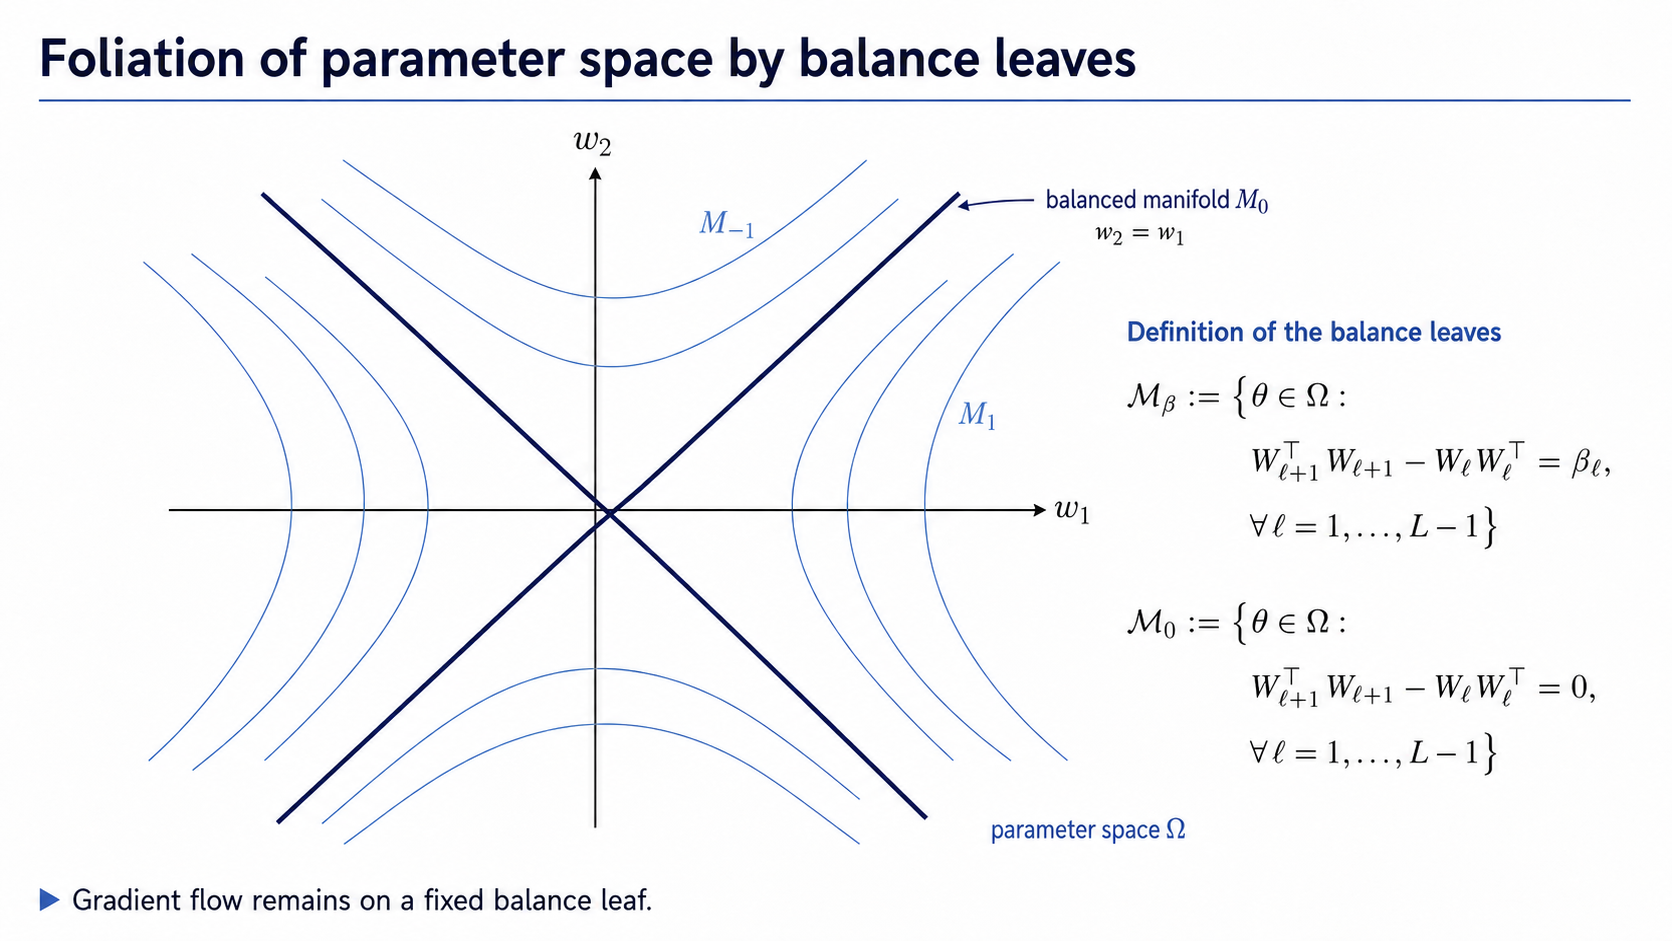
\includegraphics[width=\textwidth,height=\textheight,keepaspectratio]{figures/foliation_paramaters_balanced.png}
\end{frame}
\begin{frame}[plain]
\centering
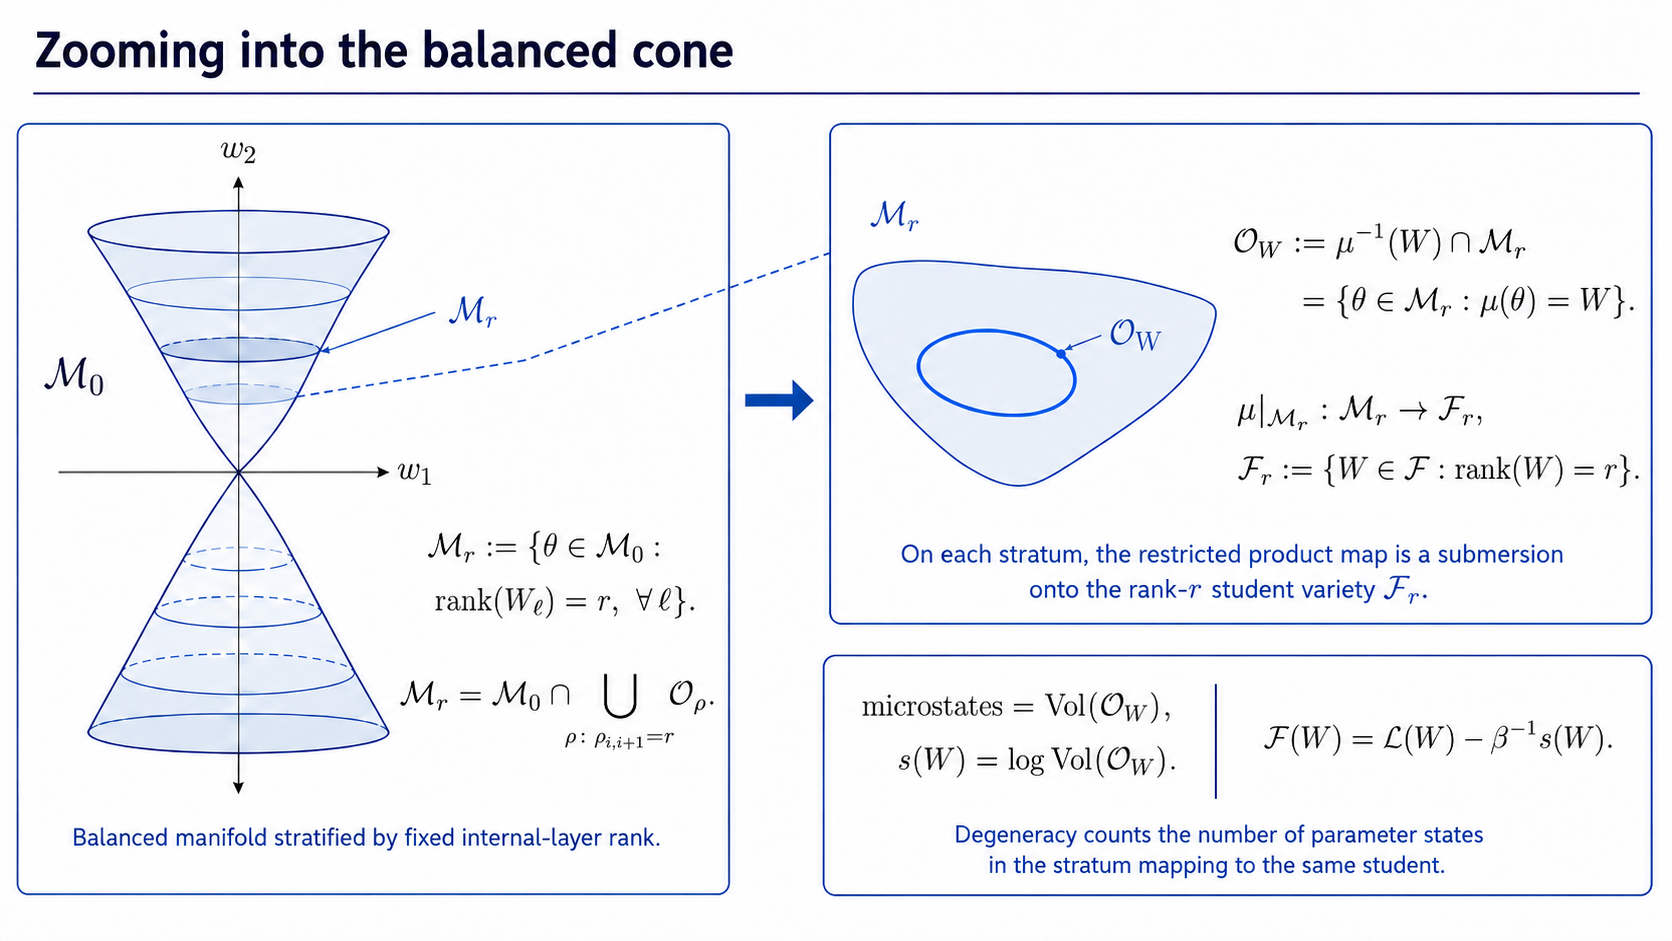
\includegraphics[width=\textwidth,height=\textheight,keepaspectratio]{figures/balanced_cone_micro_states.pnd.png}
\end{frame}
\begin{comment}
\begin{frame}{Foliation of the balance manifold}
    The conserved balanced quantities
\[
B_\ell(\theta)
=
W_{\ell+1}^{\top}W_{\ell+1}
-
W_\ell W_\ell^{\top}
\]
define level sets
\[
\mathcal M_G = B^{-1}(\beta).
\]
Thus parameter space decomposes as
\[
\Omega=\bigsqcup_G \mathcal M_G.
\]
Since \(\frac{d}{dt}B_\ell(\theta(t))=0\) along gradient flow, each flow is contained
\(\mathcal M_G\) is invariant through the flow.
\end{frame}
\begin{frame}
    \begin{block}{Rank strata inside the balanced leaf}
On the balanced leaf \(\mathcal M_0\),
\[
    W_{\ell+1}^{\top}W_{\ell+1}
    =
    W_\ell W_\ell^{\top}.
\]
Hence consecutive layers have the same singular values, and therefore the same rank.
Thus
\[
    \mathcal M_0
    =
    \bigsqcup_r \mathcal M_r,
    \qquad
    \mathcal M_r
    :=
    \{\theta\in\mathcal M_0:\operatorname{rank}(W_\ell)=r\ \forall \ell\}=\mathcal M_0 \cap \mathcal{O}_{\rho_{i,i+1} = r}
\]
Moreover,
\[
    \mu(\mathcal M_r)
    =
    \mathcal F_r
    :=
    \{W\in\mathcal F:\operatorname{rank}(W)=r\}.
\]
Balanced rank-\(r\) parameter leaf projects to the rank-\(r\) stratum of
function space.
\end{block}
\end{frame}
\end{comment}
\begin{frame}{The manifold of gradient flow}
Gradient flow is constrained on the following hyperbolic manifold:
\begin{equation*}
    \mathcal{M}_{\beta} := \{\theta\in\Omega| W_{l+1}^{\top}W_{l+1} - W_{l}W_{l}^{\top} = \beta_l\}
\end{equation*}
\begin{block}{Gradient flow on the balanced variety}
On the balanced variety $\mathcal{M}_0$, self consistent gradient flow equation in function space:
\begin{equation*}
    \dot{W}
    =
    \sum_{k=1}^{L}
    (WW^{\top})^{\frac{L-k}{L}}
    R(W)
    (W^{\top}W)^{\frac{k-1}{L}},
    \qquad
    R(W):=\Sigma_{YX}-W.
\end{equation*}
For depth $2$:
\[
    \mathcal{M}_0
    =
    \{(W_1,W_2)\mid W_2^{\top}W_2=W_1W_1^{\top}\}.
\]
\begin{equation*}
    \dot{W}
    =
    (WW^{\top})^{\frac{1}{2}}R(W)
    +
    R(W)(W^{\top}W)^{\frac{1}{2}}.
\end{equation*}
\end{block}
\end{frame}
\begin{frame}[plain]
\centering
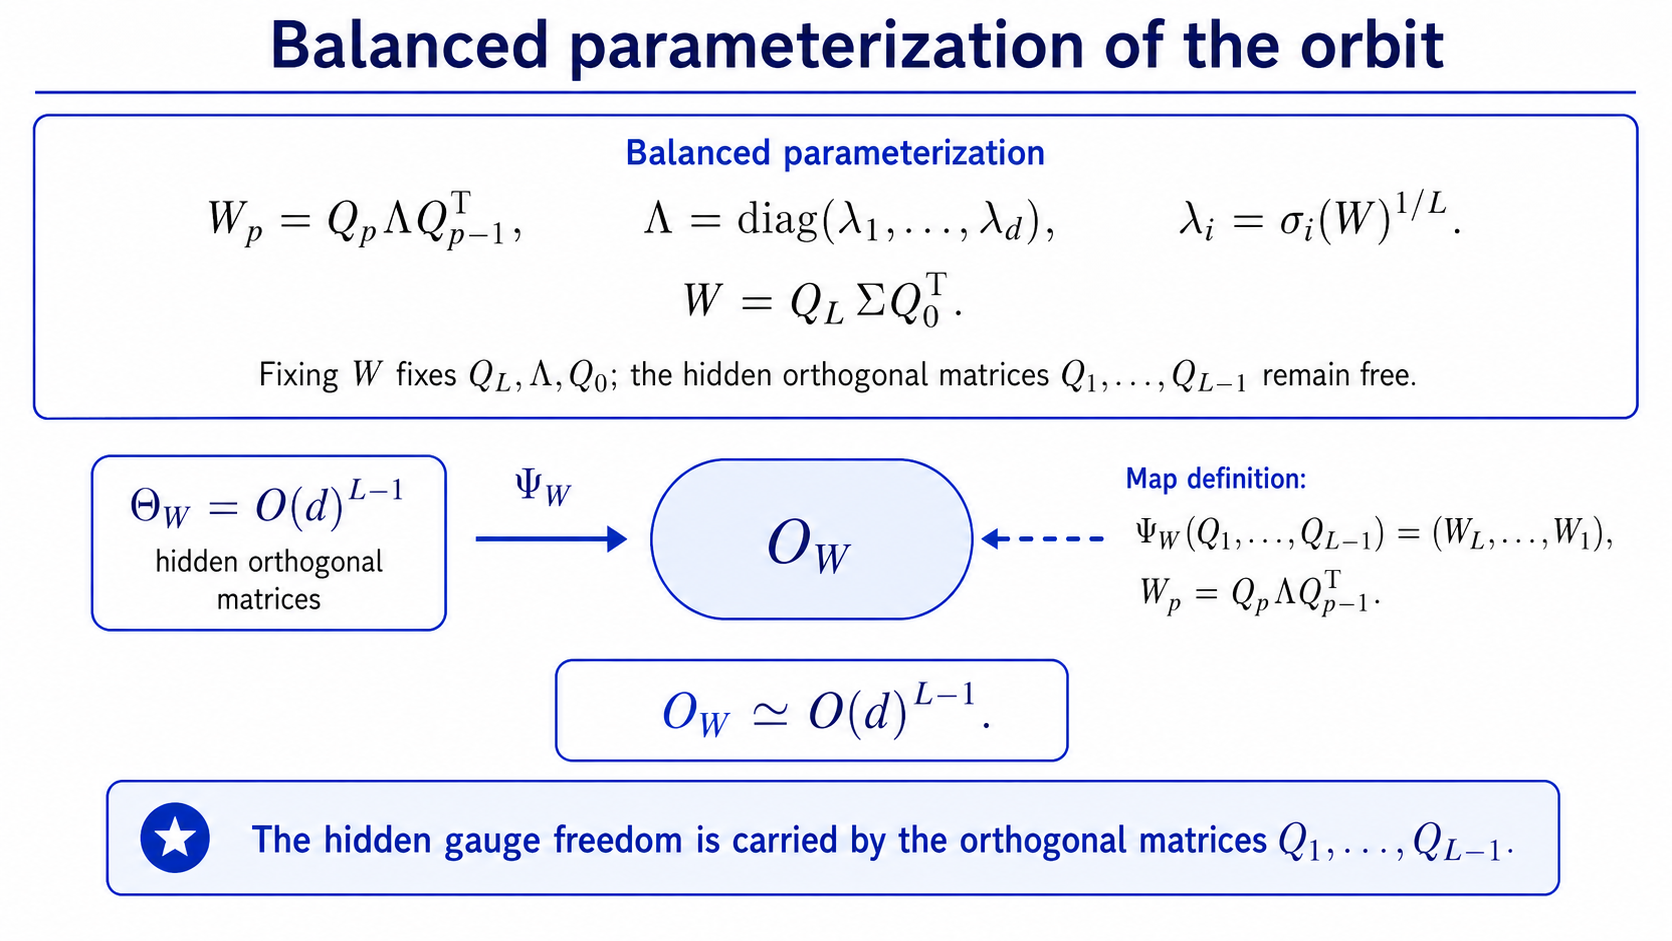
\includegraphics[width=\textwidth,height=\textheight,keepaspectratio]{figures/balanced_parametrization.png}
\end{frame}
\begin{comment}
\begin{frame}[plain]
\centering
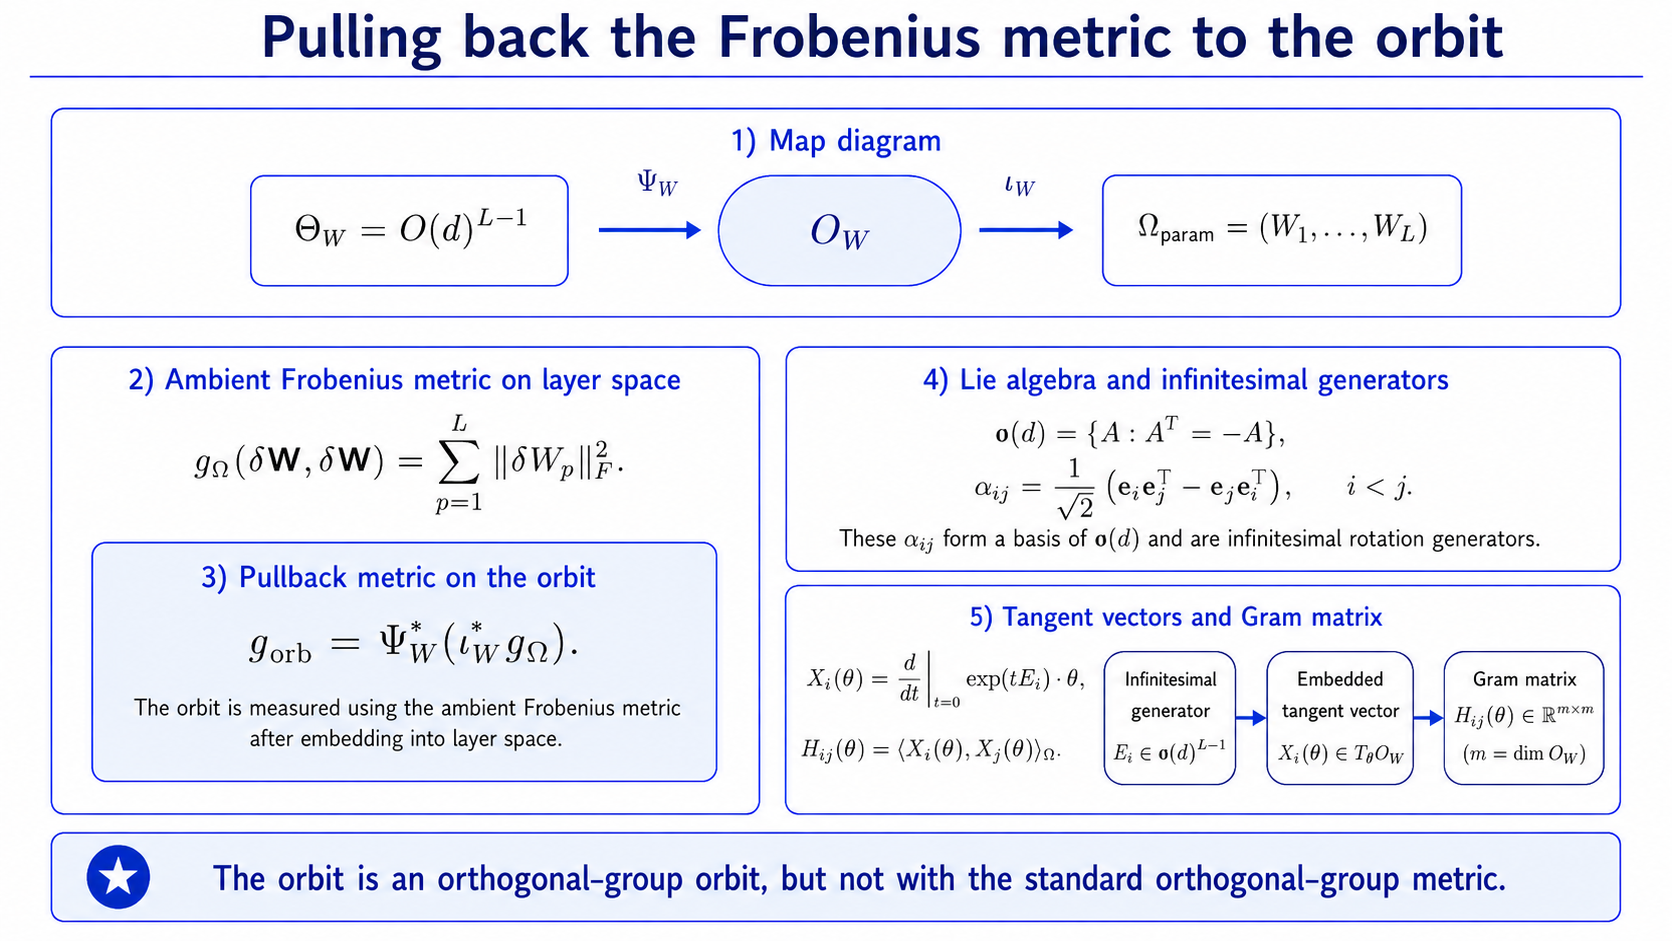
\includegraphics[width=\textwidth,height=\textheight,keepaspectratio]{figures/frobenius_pull_back.png}
\end{frame}
\end{comment}
\begin{frame}[plain]
\centering
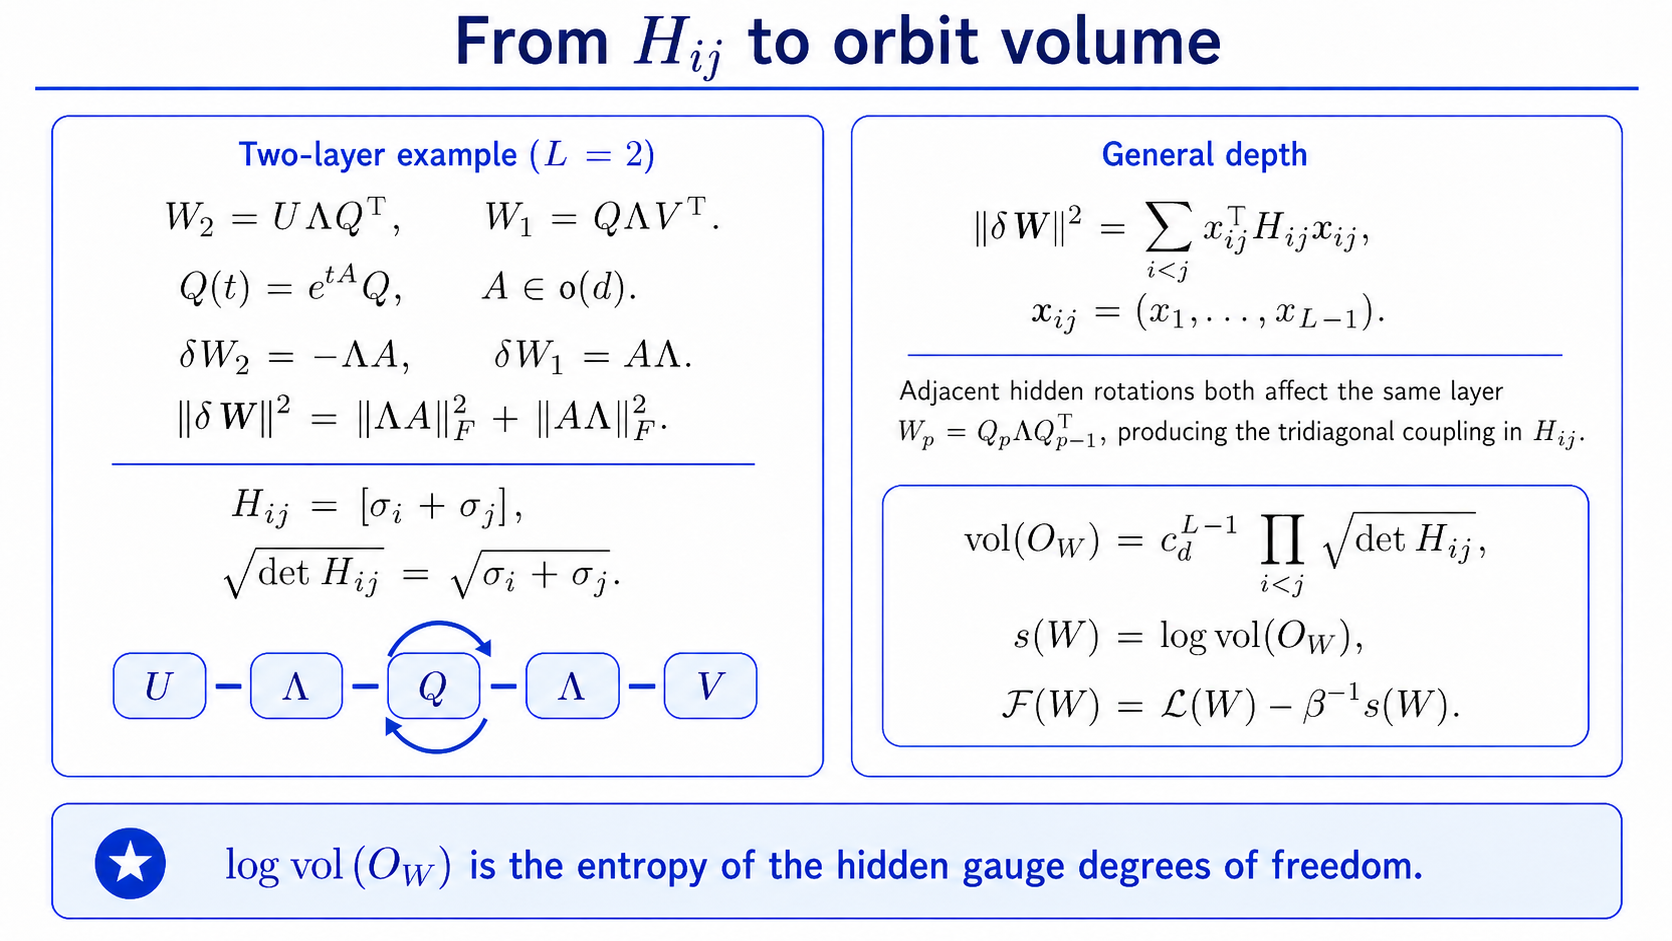
\includegraphics[width=\textwidth,height=\textheight,keepaspectratio]{figures/orbit_volume.png}
\end{frame}
\begin{comment}
\begin{frame}{Riemannian flow}
    \begin{block}{Why the projected flow is Riemannian}
On a balanced rank stratum \(\mathcal M_r\), the product map
\[
    \mu:\mathcal M_r\to\mathcal F_r
\]
is a Riemannian submersion when \(\mathcal F_r\) is equipped with the induced metric
\[
    \|Z\|_{g_L,W}^2
    =
    \min_{D\mu_\theta[\dot\theta]=Z}
    \sum_{\ell=1}^L \|\dot W_\ell\|_F^2 .
\]
Since \(\mathcal L\circ\mu\) is constant along the fibers of \(\mu\), its Euclidean gradient is
horizontal. Therefore
\[
    D\mu_\theta[\nabla_\theta(\mathcal L\circ\mu)]
    =
    \operatorname{grad}_{g_L}\mathcal L(W),
\]
and the parameter gradient flow projects to
\[
    \dot W=-\operatorname{grad}_{g_L}E(W).
\]
\end{block}
\end{frame}
\begin{frame}
    \begin{block}{From energy to free energy}
The product map has fibers
\[
    \mathcal O_W:=\mu^{-1}(W)\cap\mathcal M_r ,
\]
i.e. many parameter microstates represent the same function \(W\).
Their volume defines a Boltzmann entropy
\[
    S(W):=\log\operatorname{vol}(\mathcal O_W).
\]
With microscopic fluctuations along the fibers, the effective macroscopic objective is
\[
    F_\beta(W)=E(W)-\frac1\beta S(W).
\]
Thus the Riemannian energy flow is replaced by free-energy flow:
\[
    \dot W=-\operatorname{grad}_{g_L}F_\beta(W)
    =
    -\operatorname{grad}_{g_L}E(W)
    +\frac1\beta\operatorname{grad}_{g_L}S(W).
\]
\end{block}
\end{frame}
\end{comment}
\begin{comment}
\begin{frame}{Spectral entropy on the balanced manifold}

Balanced layers have the same singular values
\[
\lambda_1,\dots,\lambda_d,
\qquad
\sigma_i=\lambda_i^L.
\]
\begin{block}{Entropy}
Boltzmann entropy of orbit:
\[
S(W):=\log \operatorname{vol}(\mathcal O_W).
\]
Menon formula:
\[
S(W)
=
(L-1)\log c_d
+
\frac12\sum_{i<j}
\log\!\left(
\frac{\lambda_i^{2L}-\lambda_j^{2L}}
     {\lambda_i^2-\lambda_j^2}
\right).
\]
\end{block}

\end{frame}
\end{comment}
%----------Rich Regime for DLNs-----------
\begin{frame}{Rich regime in DLNs}
Assume whitened inputs $\Sigma_X = I$ and $\Sigma_{YX} = U S V^{\top}$. Define a 2-layer DLN layerwise-modes as:
\begin{equation*}
    w_1^{\alpha} := W_1 v^{\alpha} \in \mathbb{R}^{d_1}, 
    \qquad
    w_2^{\alpha} := W_2^{\top} u^{\alpha} \in \mathbb{R}^{d_1},
\end{equation*}
We have the DLN's mode matrix:
\begin{equation*}
    w_{\alpha\beta}=u^{\alpha\top} W_2 W_1 v^{\beta} = (w_2^{\alpha})^{\top} w_1^{\beta}.
\end{equation*}
Assuming gradient flow on the balanced manifold, using the self-consistent GF equation:
\begin{equation*}
    \dot{w}_{\alpha\alpha} = 2\left(s_{\alpha} - w_{\alpha\alpha}\right)w_{\alpha\alpha}
    - 2\sum_{\beta\neq\alpha} \left(w_{\alpha\beta}\right)^2 .
\end{equation*}
\end{frame}
\begin{frame}{Rich regime in DLNs}
We neglect the cross-mode terms $w_{\alpha\beta}$ (weights are aligned).
\begin{block}{Logistic feature learning}
    For balanced and aligned weights, GF reduces to a system of 1D logistic ODEs:
\begin{equation*}
    \dot{w}_{\alpha} = 2\left(s_{\alpha} - w_{\alpha}\right)w_{\alpha}.
\end{equation*}
Solving this ODE for $w(t):=w_{\alpha}$ gives:
\begin{equation*}
    w(t)=\frac{s}{1+\left(\frac{s}{w_0}-1\right)e^{-2s t}}.
\end{equation*}
\end{block}
\end{frame}
\begin{frame}{Time scale of learning in the rich regime}
 The elapsed time to go from $w_0$ to $w_f$ is
\[
t=\frac{1}{2s}\,\ln\!\left(\frac{w_f\,(s-w_0)}{w_0\,(s-w_f)}\right), \qquad s\neq 0.
\]
For depth $L$:
\[
t=\frac{1}{L} \left[ \frac{1}{s^{2}} \ln\!\left(\frac{w_f\,(s - w_0)}{w_0\,(s - w_f)}\right)
+ \frac{1}{s\,w_0} - \frac{1}{s\,w_f} \right].
\]
\begin{block}{Rich regime}
\begin{itemize}
    \item Stagewise learning ordered by the magnitude of singular values
    \item Saddle to saddle dynamics: GF goes from low to high rank saddles
    \item Simplicity bias of gradient flow and low-hanging fruit prior
\end{itemize}
\end{block}
\end{frame}
%----------Lazy Regime for DLNs-----------
\begin{frame}{Linear regime in DLNs}
\begin{block}{Proposition}
For a DLN of depth $L$ in the large width limit, or with a large initialization, we have:
    \begin{align*}
    \dot{W} & \approx K_0[M - W]
\end{align*}
Leading to the following solution:
\begin{equation*}
    W(t) = M - \exp(-K_0 t)[M - W(0)]
\end{equation*}
\end{block}
The time scale of learning is mostly fixed by the NTK at initialization:
\begin{equation*}
    t \approx -k_0^{-1}\log\left(\frac{s - w_f}{s - w_0}\right)
\end{equation*}
No stagewise learning, the structure of the data barely influences the training dynamics, behaves like a linear network.
\end{frame}
\begin{frame}
    TODO
\begin{itemize}
    \item References Slides
    \item Langevin Dynamics slide
    \item Discussion Slide
    \item Make nicer slides for intro
\end{itemize}
\end{frame}
\end{document}
